\documentclass[conference]{IEEEtran}
\IEEEoverridecommandlockouts
% The preceding line is only needed to identify funding in the first footnote. If that is unneeded, please comment it out.
\usepackage{cite}
\usepackage{amsmath,amssymb,amsfonts}
\usepackage{algorithmic}
\usepackage{graphicx}
\usepackage{textcomp}
\usepackage{xcolor}
\def\BibTeX{{\rm B\kern-.05em{\sc i\kern-.025em b}\kern-.08em
    T\kern-.1667em\lower.7ex\hbox{E}\kern-.125emX}}
\usepackage{color}

\definecolor{dkgreen}{rgb}{0,0.6,0}
\definecolor{gray}{rgb}{0.5,0.5,0.5}
\definecolor{mauve}{rgb}{0.58,0,0.82}

\usepackage{listings}             % Include the listings-package
\lstset{frame=tb,
  language=Java,
  aboveskip=3mm,
  belowskip=3mm,
  showstringspaces=false,
  columns=flexible,
  basicstyle={\small\ttfamily},
  numbers=none,
  numberstyle=\tiny\color{gray},
  keywordstyle=\color{blue},
  commentstyle=\color{dkgreen},
  stringstyle=\color{mauve},
  breaklines=true,
  breakatwhitespace=true,
  tabsize=3
}
\begin{document}

\title{Assignment \#5\\
{\footnotesize CPEN 442}
}

\author{
\IEEEauthorblockN{Ben Henaghan}
\IEEEauthorblockA{\textit{Department of Electrical and Computer Engineering} \\
\textit{University of British Columbia}\\
Vancouver, Canada \\
Student Number: 96671466}
\and
\IEEEauthorblockN{Scott Wang}
\IEEEauthorblockA{\textit{Department of Electrical and Computer Engineering} \\
\textit{University of British Columbia}\\
Vancouver, Canada \\
Student Number:  72573322}
\and
\IEEEauthorblockN{Austine Yapp}
\IEEEauthorblockA{\textit{Department of Electrical and Computer Engineering} \\
\textit{University of British Columbia}\\
Vancouver, Canada \\
Student Number:  86705340}
\and
\IEEEauthorblockN{Mike Yue}
\IEEEauthorblockA{\textit{Department of Electrical and Computer Engineering} \\
\textit{University of British Columbia}\\
Vancouver, Canada \\
Student Number:  24583156}
}

\maketitle

\section{PROBLEM \#1}
Selected malware: Dridex
\subsection{Analyze the design of the picked malware, i.e., its structure, behavior, mechanisms it uses for selecting victims, infecting them, hiding itself and its authors, etc.}
Dridex is a type of banking trojan that specialises in stealing bank credentials and other personal information through HTML injections. The malware mainly targets customers of major online banking/financial institutions based in Europe. The spread of Dridex utilises social engineering by sending seemingly harmless Microsoft Office documents via email to unsuspecting victims. When a target opens the email attachment and allows the use of Microsoft Office macros, the macro downloads the main payload of the virus, the Dridex malware, which installs and runs on the victim’s computer. Once installed on an infected system, an adversary may execute various actions such as:
\begin{itemize}
\item Upload files
\item Download files
\item Execute files
\item Monitor network traffic
\item Browser screenshot taking
\item Add the compromised computer to a botnet
\item Communicate with other peer nodes through the peer-to-peer (P2P) protocol to retrieve configuration details
\item Download and execute additional modules
\item Download and execute additional files
\item Inject itself into browser processes for Internet Explorer, Chrome, and Firefox in order to monitor communications and steal
 information.
\end{itemize}
Dridex employs the following network infrastructure, as shown in Fig.~\ref{fg1}.
\begin{figure*}[h]
\centerline{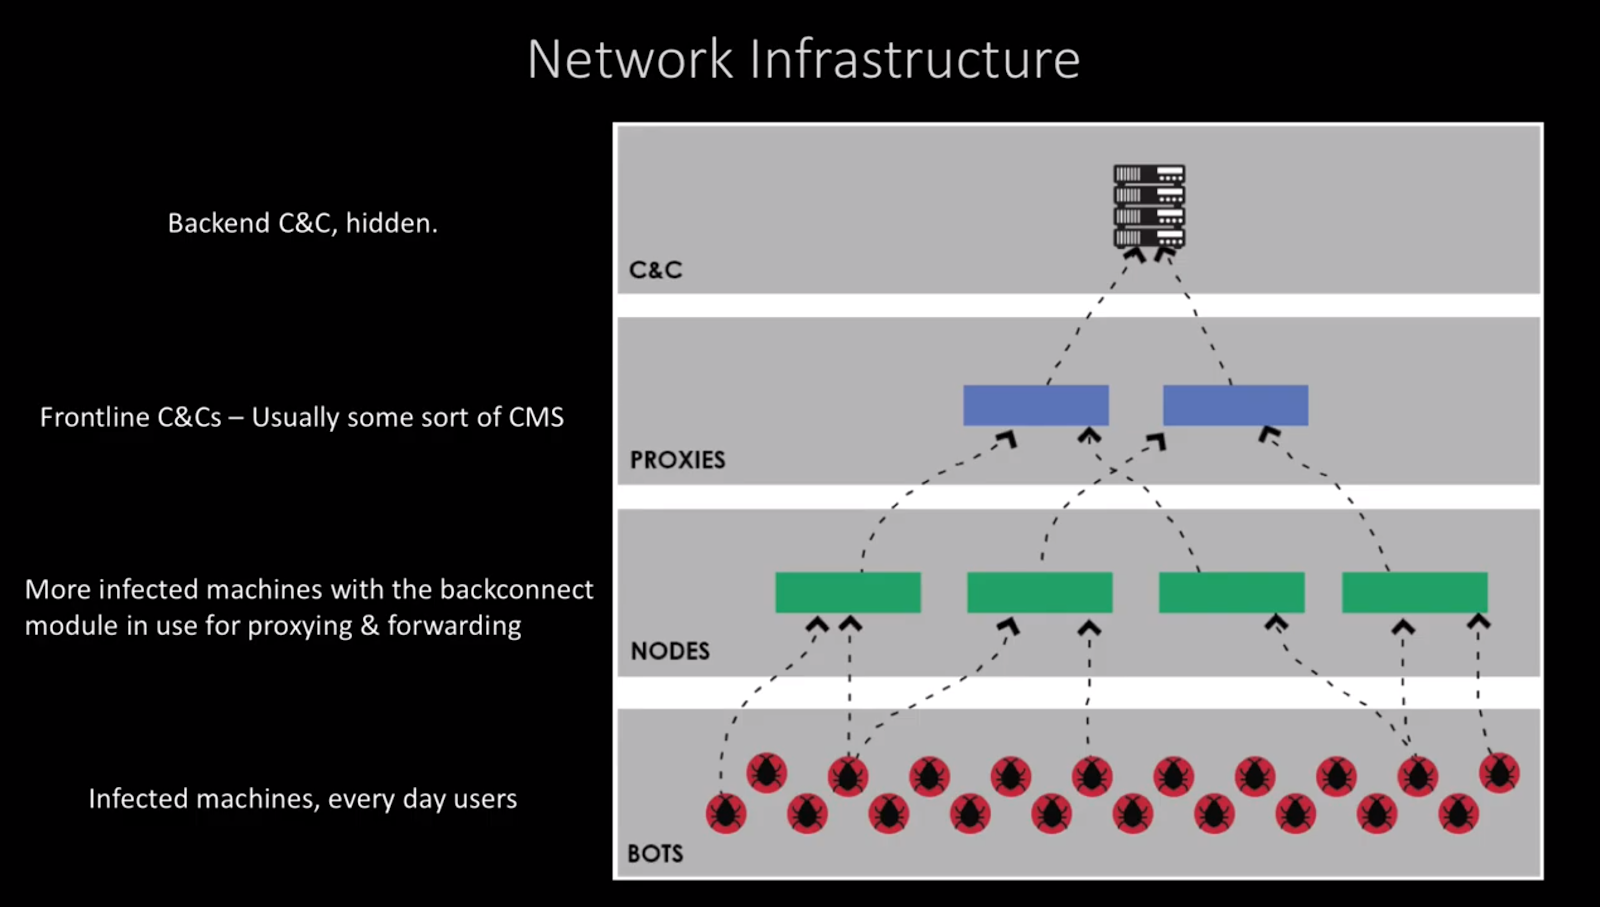
\includegraphics[width=\textwidth]{img/dridex_network_infrastructure.png}}
\caption{Network infrastructure of Dridex}
\label{fg1}
\end{figure*}

In most instances, the victim's bank credentials are compromised through keystroke monitoring or taking a screenshot during an internet banking session. Although Dridex is most commonly associated as being a banking trojan used for stealing online banking credentials, it also has the ability to redirect HTTP traffic, steal cookies, steal form data, etc. This could potentially lead to further privacy violations of other online accounts such as social media.

Dridex has been constant updated with new capabilities. In recent times, changes have been made to Dridex that aim to avoid detection by anti-virus systems. Anti-virus software mainly rely on incompatible file signatures (MD5 or SHA256 hashes) to detect malicious files. To avoid detection, Dridex leverages on newly created and signed 64-bit dynamic link libraries (DLLs), which have different file signatures from their earlier versions. These DLLs are side loaded via legitimate Microsoft Windows binaries and appear to be part of a legitimate software product, making detection even more difficult.

Dridex malware is an evolution of the Cridex malware that is based on the ZeuS Trojan Horse malware, and is distributed by the Necurs botnet. 

\subsection{Identify the aspects specific to your malware that can be used to detect or prevent it}
Firstly, the Dridex malware is spread through malicious Microsoft Office documents. As such, only users of Windows computer may be affected; Dridex cannot install itself on other PC operating systems, such as macOS or Chrome OS, nor can it load on mobile operating systems, such as iOS and Android. 
 
Furthermore, Dridex utilises Microsoft Office macros to infect its victims. Users should thus disable macros in Microsoft Office and be careful of opening Word and Excel file attachments sent from unrecognised email addresses.

\subsection{Based on your analysis, recommend short, medium and long term countermeasures (i.e., protection and detection techniques) against the threat posed by this malware.}
Short term countermeasure: 
If DRIDEX infection is suspected or detected, immediately change the online banking account passwords using a different (and hopefully uninfected) system, and touch base with the bank to alert them for any fraudulent transactions taking place. Do the same for any account that you may have accessed using your infected system.
 
Medium term countermeasure:
Delete any suspicious-looking emails you receive, especially if they sport links and/or attachments. Don’t even open them, just delete them. If they purport to come from legitimate organizations, verify with the organization in question first.
 
Long term countermeasure:
Install an antimalware solution that also covers email in its protective scope. This should remove the chance of you accidentally opening malicious email/malicious attachments in the first place.

\section{PROBLEM \#2}
We wrote the solution steps of some lessons that we have solved it but the icon didn't turn to green.
\subsection{General: Google Chrome Developer Tools}

Lesson 4:
\begin{enumerate}
\item  Used the console in the dev tools and call the javascript function webgoat.customjs.phoneHome()
\item Got the random number in console: 669788521
\end{enumerate}

Lesson 6:
\begin{enumerate}
\item  Used the network tool in the dev tools to capture the request
\item Found the network number: 36.45863852087676 in data section.
\end{enumerate}

\subsection{Injection Flaws: SQL Injection(advanced)}
Lesson 3:
\begin{enumerate}
\item  Used SQL injection: 
\begin{equation}
Dave'; SELECT * FROM user\_system\_data;--
\end{equation}
\item We can find the password of Dave in the tables showed after injection, which is: passW0rD
\end{enumerate}

Lesson 5:
\begin{enumerate}
\item  First of all, try to register with the following username: Tom' AND '1'='1, and find that the user name is taken.
\item So we can use this method to check what tom's password is one at time by registering the following username: Tom' AND substring(password,1,1)='t
\item By checking all the remaining charactersm we found the password, thisisasecretfortomonly.
\end{enumerate}

\subsection{Injection Flaws: SQL Injection(mitigation)}
Lesson 6:

Below is the code I used for this lesson: 
\begin{lstlisting}
try {
	Connection conn = DriverManager.getConnection(DBURL, DBUSER, DBPW);
	PreparedStatement stmt = conn.prepareStatement("SELECT * FROM users WHERE name = ?");
	stmt.setString(1, "Scott");
	stmt.executeUpdate();
} catch (Exception e) {
    System.out.println("Oops. Something went wrong!");
}
\end{lstlisting}
I believed there is no problem of this code but when I submit the code, it showed: "error while writing TestClass: /TestClass.class"

\subsection{Authentication Flaws: Password reset}
Lesson 6:

I followed the link to change the request host from webwolf.ece.ubc.ca to webgoat.ece.ubc.ca and successfully catched the request from WebWolf. However, the value of path field in the request doesn't contain the correct path for resetting the password. I suspect the server didn't send the correct link to Tom for resetting password.

\begin{thebibliography}{00}
\bibitem{b1} F. Stroud, “Dridex malware,” webopedia. [Online]. Available: https://www.webopedia.com/TERM/D/dridex-malware.html\#. [Accessed: 05-Nov-2019].
\bibitem{b2} M. Sanghavi, “RIDEX and how to overcome it,” Symantec Official Blog, 30-May-2015. [Online]. Available: https://www.symantec.com/connect/blogs/dridex-and-how-overcome-it. [Accessed: 05-Nov-2019].

\end{thebibliography}
\end{document}
